\chapter{Introduction}
\graphicspath{{introduction/figs}}

\section{Tipping Points}
Take a pan of water and heat it up. As its temperature rises, some of the water's properties may change. For example, the viscosity and heat flux to the
environment may change. However, the water still remains as water and these changes will vary continuously with the water temperature. However, if the water is heated beyond
a critical temperature of \SI{100}{\degreeCelsius} something more dramatic happens and the water boils away. The properties of the resulting steam are quite different
to the original water --- a \emph{qualitative} change has occurred.

It is this sort of qualitative change that this thesis shall be concerned with. Whilst the boiling of water is a phase transition \parencite{Goldenfeld1992}, I shall use the broader terminology
of \emph{tipping points} \parencite{Lenton2008} or \emph{critical transitions} \parencite{Rahmstorf1995} or \emph{abrupt changes} \parencite{Alley2003} to describe these phenomena. I shall largely stick
to the term tipping point, or just tipping, which has its origins in the idea that when an object is lent over it will return to its original position unless it is lent over sufficiently far when the object
will tip over.

\subsection{Definitions}

Although it can be a vague term, the concept of a small nudge leading to a large change generally forms a part of most formal definitions of tipping points.
For example,~\cite{Lenton2008} defines the occurrence of a tipping
point as when a control parameter, there is a critical value $\rho_{\mathrm{crit}}$ of a control parameter, $\rho$, above which any significant variation, $\delta \rho > 0$ leads to a qualitative change
$\hat{F}$ of a system feature $F$, after some observation time $T > 0$. They write this mathematically as
\begin{equation}
  \label{eq:lenton_tipping_definition}
  |F(\rho \geq \rho_{\mathrm{crit}} + \delta \rho | T) - F(\rho|T)| \geq \hat{F} > 0.
\end{equation}
More recently,~\cite{ArmstrongMcKay2022} updated this definition by requiring $\delta \rho$ to be within the natural variability of the system. They also require that changes become self perpetuating
beyond $\rho_{\mathrm{crit}}$ as a result of the asymmetry of relevant feedbacks and that the tipping leads to `substantial' impacts. The IPCC \parencite{AR6} defines tipping differently still
as `a level of change in system properties beyond which a system reorganises, often in a nonlinear manner, and does not return to the initial state even if the drivers of the change are abated'.
Others, such as~\cite{Wang2023}, inspired by~\cite{Kopp2016}, insist that tipping points should occur on fast time scales.

Each of these definitions are deficient in their own way. The IPCC definition allows for linear behaviour, although tipping is a fundamentally nonlinear phenomenon. It also insists on \emph{hysteresis},
which is the property that the system does not return to its initial state after abating the drivers, although not all examples of tipping --- including boiling water --- experience this.
The complex definition in~\cite{Lenton2008} views tipping in terms of changes in parameters of a system, and not something a system can do spontaneously, which excludes certain types of
tipping (see \cref{sec:tipping_typology}). The third definition, that of~\cite{ArmstrongMcKay2022}, suffers from the problems of~\cite{Lenton2008} and also requires `substantial' impacts, which
artificially restricts the abrupt shifts that can be investigated. Finally,the requirement of~\cite{Wang2023} that tipping points be realised quickly is problematic for Earth System investigations
as some of the tipping points of interest will be realised slowly.

In this thesis, I will use the term tipping point in the sense that a system undergoes a tipping point when it experiences a qualitative change in its properties. Although this is a vague definition,
it enables the term tipping point to include all dynamics of interest. I am adopting Potter Stewart's philosophy that although a tipping point might be hard to define,
`I know it when I see it' \parencite{Stewart1964}.

\subsection{Examples of Tipping}

These sorts of nonlinear changes have long fascinated scientists. Physicists have investigated phase changes not just in terms of the boiling and freezing of substances but also
in magnetic materials \parencite{Ising1925,Onsager1944}, superconductivity \parencite{Landau1965} and percolation theory \parencite{Flory1941}. Each of these are different processes, but it is a
remarkable fact that near the phase transition different systems can be dynamically very similar, a phenomenon known as universality \parencite{Wilson1983}. This sort of idea --- that different examples
of tipping points across totally different systems can share many common features as been an important driving force in the theory of tipping points. 

Tipping points are also important in biology. In medicine, tipping point theory has been used to help understand asthma attacks \parencite{Donovan2022} and sleeping dynamics \parencite{Skeldon2014}.
Tipping points have proven very important in ecology. In an influential article, \parencite{May1976}, the ecologist Robert May noted that even very simple nonlinear models have rich dynamics and are capable
of experiencing tipping points (although he did use that term).~\cite{Holling1973} introduced the idea of resilience which is to do with the ability of a system to resist tipping. Tipping points have
been found in a range of ecosystems \parencite{Scheffer2001,Dakos2019}. The transition to turbid state in lakes \parencite{Scheffer1993} and the collapse of plant-pollinator communities
\parencite{Lever2014} are both examples of ecological tipping points, however other studies \parencite{Hillebrand2020} have challenged this.

Notions of multiple equilibria and the ability to transition between them has been used to explain patterns seen in nature. This was introduced by Turing \parencite{Turing1952} to explain
patterns found in certain plants and animals. Since then, it has been used to explain patterns in ecosystems \parencite{Rietkerk2008}.

\section{The Climate-Carbon System}

Whilst part of this thesis is applicable to many systems, the focus of this work has been on applications to the Earth system. Therefore in this section I will give an outline in
how the climate-carbon system operates.

The fundamental idea in climate science is that of energy balance \parencite{North1981}. The Earth recieves radiation from the Sun and then reradiates it to space.
In order to reach a steady state, the energy absorbed from the Sun must equal the radiation emitted from the Earth \parencite{Peixoto1992}. The need for energy balance, combined with the
latitudinally dependent absorbtion and emission of radiation, that ultimately drives all weather and climate \parencite{Lorenz1967}.

The solar constant, $S_0 \approx \SI{1360}{\watt\per\meter\squared}$ \parencite{Johnson1954} is the amount of radiation receieved by the Earth per unit area.  A fraction of this,
called the albedo $\alpha \approx 30\%$, is reflected back to space \parencite{Goode2021}. The rest is absorbed, mostly by the Earth's surface \parencite{Trenberth2009}.

Let the amount of radiation the Earth emits per unit area be $F$. The Earth absorbes energy in a disk of radius $R$, the Earth's radius, and reradiates
over the entire surface of the Earth. By energy balance this leads to
\begin{equation}
  \pi R^2 S_0 (1-\alpha) = 4 \pi R^2 F
\end{equation}
or
\begin{equation}
  \label{eq:energy_balance}
  F = \frac{1}{4} S_0 \left(1 - \alpha\right).
\end{equation}
Assuming the Earth radiates as a black body with temperature $T$, $F = \sigma T^4$ then $T = \SI{255}{\kelvin}$, not far from the true temperature of about \SI{287}{\kelvin} \parencite{Jones1999}.
It is however the effective emission temperature of the Earth. The difference between this and the true temperature is due to the Greenhouse effect. This is when certain atmospheric gases,
such as \ce{CO2} and \ce{H2O}, absorb outgoing radiation from the Earth's surface
but reradiate it back to space. As temperatures in the atmosphere decrease with height this lowers the effective emmision temperature of the Earth and so the Earth's surface must be
warmer than it would be in the absence of greenhouse gases to maintain energy balance. \parencite{Pierrehumbert2010}.

\subsection{Climate Response to Radiative Forcing}
When greenhouse gases are emitted into the atmosphere they reduce the amount of outgoing radiation. As less radiation is now
emitted to space the Earth's climate responds to restore equilibrium. It does this by warming up to increase the amount it of energy
radiates until it reaches equilibrium \parencite{Manabe1967,Pierrehumbert2010}. 

The amount that a greenhouse gas decreases the outgoing radiation to space by is known as its radiative forcing. Let $T$ be
the global mean temperature and assume that $N$, the net radiation received by the Earth, depends on $T$. After emitting a greenhouse gas
the change in the top of atmosphere energy flux can split \parencite{Gregory2004} into a forcing term, $\Delta Q$, and feedback term, $\lambda \Delta T$
\begin{equation}
  \label{eq:deltaN}
  \Delta N = \Delta Q - \lambda \Delta T.
\end{equation}

The climate responds to the forcing by changing its temperature so that $\Delta N$ is zero. Hence the change in global mean temperatures is
\begin{equation}
  \label{eq:response_to_radiative_forcing}
  \Delta T = \frac{\Delta Q}{\lambda}.
\end{equation}
The quantity
\begin{equation}
  \label{eq:climate_sensitivity}
  \lambda = -\pdv{N}{T}
\end{equation}
known as the \emph{climate sensitivity} determines the amount of warming experienced for a given radiative forcing. This quantity is measured
in units \si{\watt\per\square\meter\per\kelvin} but it has become common to discuss $\lambda$ in terms of a given radiative forcing, $Q_{2\times}$,
the radiative forcing due to doubling the concentration of $\ce{CO2}$ in the atmosphere, giving rise to
\begin{equation}
  \label{eq:definition_of_ECS}
  \mathrm{ECS} = \frac{Q_{2\times}}{\lambda}
\end{equation}
known as \emph{Equilibrium Climate Sensitivity} which is measured in \si{\kelvin} \parencite{Charney1979}.

Implicit in this definition is the idea that $Q_{2\times}$ is well defined. It is an empirical fact that over a range of concentrations the radiative forcing
of $\ce{CO2}$ varies to a good approximation with the logarithm of its concentration \parencite{Pierrehumbert2010}, and so the notion of a radiative forcing due to doubling is well defined.
It is also usually assumed that $\mathrm{ECS}$ is a constant independent of background climate state. Whilst this appears to be a good approximation, some authors
have investigated its state dependence \parencite{Ashwin2019,Caballero2013,Bloch-Johnson2021}.

The value of $\mathrm{ECS}$ is uncertain. State of the art climate models (CMIP6) do not agree on its value, and give a range of
\SIrange{1.8}{5.6}{\kelvin} \parencite{Zelinka2020}, which represents an increase in uncertainty from CMIP5, although some authors have suggested that ECS could be even
larger \parencite{Stainforth2005}.
However, these estimates should be combined with other observational estimates, such as~\cite{Cox2018}, as well as paleoclimate records, like~\cite{Hargreaves2012}, as done by~\cite{Sherwood2020}.
This analysis of multiple lines of evidence lead the IPCC to conclude that the best estimate of $\mathrm{ECS}$ is \SI{3.0}{\kelvin} with a likely range of \SIrange{2.5}{4.0}{\kelvin} \parencite{AR6}.

\subsection{Carbon Cycle}
Of all the \ce{CO2} emitted by humans by burning fossil fuels, only around half remains in the atmosphere \parencite{Friedlingstein2022}. This is because of the terrestrial and oceanic sinks of carbon.
The response of the carbon cycle can be partitioned into a carbon-concentration feedback and a carbon-climate feedback \parencite{Friedlingstein2006}. The carbon-concentration feedback
gives the change in the carbon cycle due to increases in \ce{CO2} before temperature changes are accounted for. The carbon-climate feedback gives the changes in carbon stores due to increases
in temperature. In CMIP6 \parencite{Arora2020} the carbon-concentration feedback is $\SI{0.97\pm0.40}{\peta\gram\carbon\per\ppm}$ over land and $\SI{0.79\pm 0.07}{\peta\gram\carbon\per\ppm}$ over ocean.
The carbon-climate feedback is $\SI{-45.1\pm50.6}{\peta\gram\carbon\per\kelvin}$ over land and $\SI{-17.2\pm5.0}{\peta\gram\carbon\per\kelvin}$. This means that increases in \ce{CO2} tend to
increase carbon on the land and in the ocean, however increases in global temperature due to elevated \ce{CO2} tend to liberate carbon from the land and oceans. It should be noted
that the uncertainties are much higher over land, which reflects the different processes contributing the land and ocean carbon cycles.

\subsubsection{Terrestrial Carbon Cycle}
The terrestrial part of the carbon cycle is controlled by the biosphere \parencite{AR6}. Carbon enters the biosphere through photosynthesis, the amount of which is known as gross
primary productivity or GPP, and leaves via respiration \parencite{Jenkinson1991}. Respiration can be subdivided into \emph{autotrophic} and \emph{heterotrophic}.
These relate to respiration done by plants (which produce their own food which hence the name \emph{auto}troph) and non-plants respectively. Heterotrophic respiration
is primarily performed by soil microbial communities which decompose the organic matter deposited into the soil from plants \parencite{Singh1977}.

This means that the net carbon flux into the biosphere due to plants called \emph{Net Primary Productivity} (NPP) is given by the difference between photosynthesis and
autotrophic respiration. In the absence of other carbon removals, the overall carbon flux between the land and the atmosphere is therefore the
difference between NPP and heterotrophic respiration, known as Net Ecosystem Production (NEP). Accounting for these removals such as fire and deforestation leads to
Net Biome Productivity (NBP) which is the total flux of carbon into the land \parencite{Lovett2006,Fernandez-Martinez2023}. 

This carbon is stored in vegetation and in soils. There is around \SI{1500}{\peta\gram\carbon} in the soil, with about \SI{560}{\peta\gram\carbon} in vegetation \parencite{Crowther2019}.
The significant stores of vegetation carbon are the tropical rainforests \parencite{Malhi2006}, whereas much of the soil carbon can be found at high latitudes \parencite{Varney2020}.
Permafrost, soil which is below \SI{0}{\degreeCelsius} all year round, represents a major store of this carbon \parencite{Hugelius2014}. As it is frozen, little decomposition occurs there.
However as the Earth warms and the permafrost thaws it could represent a carbon flux of some concern \parencite{Schuur2015}.


There are important feedbacks on the land carbon cycle.
Increasing the amount of \ce{CO2} in the atmosphere increases the amount of carbon that diffuses through a plant's stomata where it can be used in photosynthesis \parencite{Farquhar1980}.
Furthermore, plants will partially close their stomata at higher \ce{CO2} levels \parencite{DeKauwe2013} which reduces the water lost through transpiration. This can be quanitified in terms of the
water use efficency (the ratio of carbon gained to water lost) \parencite{Drake1997}. This can increase the growing season in drier ecosystems \parencite{Frank2015}.
These effects mean that at higher \ce{CO2} levels NPP is expected to increase.

This \emph{\ce{CO2} fertilisation effect} has been detected in models \parencite{Friedlingstein2006,Arora2020,Wenzel2016} and observationally \parencite{Ainsworth2007,KolbySmith2016}.
It acts as a negative feedback on global warming as it tends to decrease the amount of \ce{CO2} in the atmosphere by increasing photosynthesis. This feedback is
expected to weaken with increased $\ce{CO2}$ as fewer plants become limited by \ce{CO2}, there is some observational evidence of this occurring \parencite{Wang2020}.

The decomposition of organic matter through heterotrophic respiration is a biochemical process that depends on temperature. In particular, increasing the temperature of the decomposition reaction
will increase the rate of this reaction. Hence as $\ce{CO2}$ has a warming effect the amount of respiration will increase \parencite{Jenkinson1991}. 
This means there will be a larger flux of carbon to the atmosphere and so this is a positive feedback, which has been termed the Jenkinson effect \parencite{Luke2011}.
Many biological reactions are assumed to depend exponentially on temperature, increasing in rate by a factor $Q_{10}$ for every \SI{10}{\kelvin} of warming.
It is generally thought that $Q_{10} \approx 2$ \parencite{Jones2001}.

\subsubsection{Ocean Carbon Cycle}

The ocean carbon cycle operates by different mechanisms to the terrestrial carbon cycle. Some carbon enters through runoff from the land but most of the carbon flux to the ocean comes
from diffusion from the atmosphere to the ocean \parencite{Devries2022}. This diffusion depends on the solubility of \ce{CO2} in water and
the difference in partial pressure of \ce{CO2} between the atmosphere and the ocean \parencite{Wanninkhof1992}.
The \ce{CO2} reacts with seawater to form two other species of dissolved inorganic carbon, or DIC:\@ \ce{HCO3-} and \ce{CO3^{2-}} \parencite{Dickson1987}.

Strong vertical gradients exist in DIC in the ocean, with more DIC at depth due to increased solubility at depth and the biological pump \parencite{Volk1985}. Organisms convert DIC into biomass
through photosynthesis near the surface where there is enough light. Most of this is respired near the surface but due to sinking, mixing and the migration of organisms some biomass
will make its way to the deeper ocean where it is released as DIC into the deep ocean. This transport of DIC away from the surface increases the capacity of the ocean to absorb carbon
\parencite{Sarmiento1984}.


The ocean carbon cycle will be affected by climate change. Most of these changes are related to the physical and
chemcial components of the ocean carbon cycle rather than the biological components \parencite{AR6}. As a result there is much less uncertainty about future changes in the
ocean carbon cycle relative to the terrestrial carbon cycle \parencite{Arora2020}. As more \ce{CO2} is added to the ocean, the amount of \ce{CO3^{2-}} will decrease which leads to
more \ce{CO2} remaining in its dissolved form which reduces the uptake of carbon \parencite{Egleston2010}. Furthermore the solubility of \ce{CO2} decreases with
temperature so warming which thus reduces the strength of the ocean sink \parencite{Weiss1974}. Additionally the ocean is expected to become more
stratified due to climate change which decreases vertical mixing which again reduces the uptake of \ce{CO2} \parencite{DeVries2017}. 


\section{Tipping Points in the Earth System}
In this section I will give some background on Earth system Tipping points, including outlining some mechanisms.
I will focus on a few key sub subsystems. I will then discuss some of the evidence for tipping behaviour in the Earth's past.

The most recent IPCC report \parencite{AR6} finds it `unequivocal that human influence has warmed the atmosphere, ocean and land'. Humans have done this through the release of greenhouse
gases, most importantly carbon dioxide (\ce{CO2}), and also through land use change. This has led to observable changes in the Earth's climate. Most obvious is the changes in global mean surface
temperature, with a most likely temperature increase of \SI{1.07}{\kelvin} \parencite{AR6} in the global mean but with clear regional differences \parencite{Morice2021} such as
Arctic amplification as well as more warming over land than over ocean. Other effects include rise of around \SI{0.2}{\meter} in sea levels \parencite{Frederikse2020} and increase in heavy precipitation
events \parencite{Fischer2016}.

\subsection{Tipping at the global scale}
This global warming is unprecedented in at least the last 2000 years and has caused global temperature levels not seen in the last $125,000$ years \parencite{AR6}. This naturally leads to a question
about the nature of the change the Earth system is experiencing: will it be a smooth function of increasing \ce{CO2} or is tipping behaviour possible?

A controversial paper,~\cite{Steffen2018}, considered the possibility that ongoing global warming could make the Earth transition from its current current glacial-interglacial limit cycle
state into a new `hothouse' state. This state would be defined by high temperatures and sea levels, posing challenges both to humanity and the wider biosphere. This state would be reached
through biogeochemical feedbacks leading to a cascade of tipping points. They advocate humanity operating within certain `planetary boundaries' \parencite{Rockstrom2009} to avoid this possibility.

Part of the reason~\cite{Steffen2018} proved so controversial is that there is little evidence this nonlinear response at the global scale. Global temperature rise is approximately linear
in emitted carbon dioxide \parencite{Allen2009,Rogelj2019} and not expected to continue after emissions cease \parencite{MacDougall2020}. However certain cloud resolving models
report that at sufficiently high levels of global warming stratocumulus cloud decks can break up causing \SI{8}{\kelvin} of warming globally \parencite{Schneider2019}.

\subsection{Tipping Elements}

However there is still the possibility of more regional tipping point behaviour.~\cite{Lenton2008}, introduced the notion of \emph{tipping elements} which
are components of the Earth system that are `at least subcontinental in scale' ($\mathcal{O}(\SI{1000}{\kilo\meter})$) which can undergo tipping behaviour as a result of
anthropogenic influence. Lenton lead an expert elicitation of potential tipping elements in the Earth system to estimate how much warming would be needed to trigger the tipping element
and what the key uncertainties were. More recently,~\cite{ArmstrongMcKay2022} updated this study by reviewing the literature published since.  Following this, I will discuss some key tipping elements.

\subsubsection{Atlantic Meridional Overturning Circulation}
The Atlantic Meridional Overturning Circulation, known as the AMOC, is a large-scale current in the ocean. The AMOC transports warm water polewards. This heat transport plays an
important role in the climate of, for example, northern Europe where it keeps temperatures warmer than they would be otherwise. The AMOC is driven by the salt-advection feedback, whereby
warm saline water is transported northwards where it cools and becomes more dense.  It then sinks and can make the return journey to the equator completing the circulation  \parencite{Dijkstra2011}.

The potential for the AMOC to exhibit bistability was postulated by Stommel in a pioneering paper \parencite{STOMMEL1961}. He showed in a simple two box model that if the North Atlantic was
freshened then the salt-advection feedback means that meridional transport could shift to a different state. Later work \parencite{Rahmstorf1995,Hawkins2011} found multistability in
complex ocean models, when the north Atlantic was subject to a `hosing' experiment in which fresh water was added to the oceans. Other research has shown the AMOC is sensitive to the
rate of hosing \parencite{Alkhayuon2019} in a complex way \parencite{Lohmann2021}. By this it is meant that there is no well defined critical
hosing rate but that increasing the rate will switch the rate from a dangerous to a safe one and back again. Should the AMOC tip, this would have serious impacts on British agriculture
\parencite{Ritchie2020a}, global climate \parencite{Jackson2015} and the carbon cycle \parencite{Bozbiyik2011}.


Increased Arctic precipitation, melting of the Greenland ice sheet and increases in surface temperatures all act to weaken the AMOC \parencite{ArmstrongMcKay2022}.
Over the past half century, there is evidence that the AMOC has weaken by around 15\% \parencite{Caesar2018} and might be the weakest in a millennium \parencite{Caesar2021}.
There is observational evidence of decreasing AMOC stability \parencite{Boers2021a,Michel2022}. Some CMIP5 models show AMOC tipping at low
levels of global warming \parencite{Drijfhout2015}, although most models show only a gradual decline in the AMOC, which is helps explain why the IPCC view AMOC shut-down as
being unlikely, although they view the modelled AMOCs as being unrealistically stable \parencite{AR6}.~\cite{ArmstrongMcKay2022} estimate the AMOC's threshold to be at \SI{4}{\degreeCelsius},
with a range of \SIrange{1.4}{8}{\degreeCelsius}.

\subsubsection{Ice Sheets} 
Ice sheets, found in Greenland and Antarctica are believed to be able to tip due to many feedback processes. The melt elevation feedback, which is when an ice sheet melts and
therefore loses hight, exposing its surface to warmer air, increasing the melt rate, is an important feedback \parencite{Levermann2016}. Another relevant feedback is the
marine ice sheet instability, which occurs when the grounding line of an ice sheet meets a reverse slope \parencite{Schoof2007}.

Complex ice sheet models of Antarctica \parencite{Garbe2020} show hysteresis when global temperatures are reduced. Tipping behaviour has also been observed in complex models
of Greenland \parencite{Robinson2012,VanBreedam2020,Noel2021}. There is evidence of destabilisation in Greenland \parencite{Boers2021} and~\cite{ArmstrongMcKay2022} estimate
the critical threshold to be at around \SI{1.5}{\degreeCelsius}. For Antarctica they estimate a similar threshold for the West Antarctic Ice Sheet but a higher threshold
of around \SI{8.5}{\degreeCelsius} for the East Antarctic Ice Sheet. In all these cases, the tipping dynamics are very slow, taking $\mathcal{O}(\SI{1000}{\year})$ to materialise.

\subsubsection{Amazon Rainforest}
The Amazon Rainforest is a vast store of carbon, containing around \SI{123}{\peta\gram\carbon} \parencite{Malhi2006}, and has for many years been a sink, albeit a weakening one,
of anthropogenic carbon \parencite{Brienen2015}. The vegetation exerts an important influence on its local climate.
By shading, evapotranspiration and albedo effects the rainforest affects its own temperature \parencite{Baker2019}.
Furthermore, the forest recycles its own rainfall, which acts to increase the precipitation it experiences \parencite{Spracklen2012}. It is
these feedback processes that give the potential for tipping.

Early coupled climate-carbon models \parencite{Cox2000} showed strong decreases in carbon stored in the Amazon. This dieback \parencite{Cox2004}  from a forested to a savannah state was
caused by drying in the Amazon, where 25\% of precipitation reductions over the Amazon under elevated \ce{CO2} was caused by forest feedbacks \parencite{Betts2004}.
However, Amazon dieback was found to be sensitive to the parametrisation of land surface interactions and the control climate \parencite{Huntingford2004}. Since then,
some CMIP5 models \parencite{Drijfhout2015} showed signs of Amazon dieback and CMIP6 models show examples of regional Amazon dieback \parencite{Parry2022}.

Other anthropogenic factors can cause abrupt shifts in the Amazon. An example is shifting fire regimes. Fire in the Amazon is driven by humans \parencite{UNEP2002}.
Furthermore fires occur generally below a tree cover threshold \parencite{Wuyts2017} and fires tend to decrease the tree cover so that as fires become more common in the
Amazon due to global warming \parencite{Cochrane2009} there could be a shift to a low tree cover high fire frequency regime \parencite{Wuyts2022}, behaviour
which has been seen in Dynamic Global Vegetation Models (DGVMs) \parencite{Lasslop2016}. This can be viewed
as being caused by a percolation process \parencite{Schertzer2015,Cardoso2022}.

Percolation theory has been used to understand the increasing fragmentation of tropical forests \parencite{Taubert2018}. They argued that as deforestation reduces forest area,
this causes an increase in the number of forest fragments. Based on results from percolation theory \parencite{Stauffer1994} they found tropical forests were near to the critical point.
Other work \parencite{Boers2017} has also found that deforestation in the Amazon can cause tipping as reduced transpiration of water weakens the feedbacks on the South American Monsoon system. 

There is observational evidence to believe that the Amazon is bistable, and that it is heading towards a tipping point. There exists a range of mean annual precipitation
such that Amazon tree cover can either be high or low, which is evidence of bistability \parencite{Hirota2011,Staver2011}.  Furthermore, states with lower mean annual
precipitation appear to be less stable \parencite{Ciemer2019}. There is evidence of drying in Amazonia \parencite{Ritchie2022}, which is a driver of dieback. There is now reason to
believe the Amazon is a source of carbon to the atmosphere \parencite{Gatti2021}. There is are also indications of a loss of resilience in the Amazon \parencite{Boulton2022} which is
evidence of an approaching tipping point.

\cite{ArmstrongMcKay2022} estimate Amazon dieback to occur at global warming levels of \SIrange{2}{6}{\kelvin} with a best estimate of \SI{3.5}{\kelvin} but could be lower when the impact
of deforestation is included. Furthermore, timescales involved in this tipping point ($\mathcal{O}(\SI{100}{\year})$) are the timescales of a human life, and so make this a very policy relevant
tipping point.

\subsubsection{Other Tipping Elements}
The Atlantic Meridional Overturning Circulation, ice sheets in Greenland and Antarctica and the Amazon Rainforest are three of the most important tipping elements in the Earth
system. However there are other proposed tipping elements. For example, high latitude permafrost may be at risk \parencite{Lenton2012a}, however there is debate about whether this is
a true threshold or a more continuous change \parencite{ArmstrongMcKay2022}. Climate model simulations have suggested the possibility of hydrological tipping points
\parencite{Teufel2019} would imply an increased risk of fire.

Coral reefs can have tipping behaviour, as coral death occurs at certain temperature thresholds \parencite{Frieler2013}. The tipping point occurs at around \SI{1.5}{\kelvin} of global
warming, as a result coral reefs are at high risk of tipping.

\subsection{Tipping Cascades}
In recent years, a number of scientists have investigated the possibility of tipping cascades
\parencite{Steffen2018,Wunderling2023,Wunderling2021,Rocha2018,Lenton2013a,Kriegler2009,Klose2021}.
A tipping cascade refers to situation where one tipping element tips, causing another tipping element to tip. For example, loss of Greenland ice sheets could increase
the probability of the AMOC tipping \parencite{Caesar2018,Rahmstorf2015}. However, other interactions between tipping elements might have a stabilising effect, For example,
loss of the west Antarctic ice sheet could stabilise the AMOC \parencite{Sinet2023} due an increased melt water flux.

Whilst much findings about tipping points are uncertain,
this is particularly acute in the case of research into tipping cascades where much of the research involves the use of conceptual models with highly stylised interactions between elements.
However, although many researchers would  regard these tipping elements and tipping cascades as unlikely to be triggered, they are often considered `too risky to bet against' \parencite{Lenton2019a}.
The concept of being too risky to bet against relates to the fact
that catastrophic events dominate the costs in a cost benefit analysis \parencite{Weitzman2009} as long as they have a non-negligible probability of occurring.
To demonstrate that these events can occur, I will give some examples of abrupt shifts from the Earth's past.

\subsection{Evidence of Tipping Points from Paleoclimate}
The Earth is about four and a half billion years old \parencite{Dalrymple2001}, and over that time the Earth has experienced many different climates \parencite{Alley2003}.
These climates are reconstructed using proxy data. For example, \ce{CO2} concentrations found in Antarctic ice cores can be used to estimate atmospheric \ce{CO2} levels for the
last $800,000$ years \parencite{Bereiter2015}. Other methods, for example using isotopic data, can be used to reconstruct even older climates \parencite{Tierney2020}.

When examining the time series these reconstructions generate, some abrupt shifts can be seen \parencite{Boers2022,Brovkin2021}. Although it is challenging to work out if these
shifts represent tipping points or continuous change \parencite{Brovkin2008}, there is evidence that some of these shifts are examples of tipping \parencite{Dakos2008}.
Three example abrupt shifts are considered here.
The Snowball Earth is considered as an example of a global shift, Dansgaard-Oeschger events as an example of a rapid abrupt shift and the Green Sahara as an example of a abrupt shift in
the biosphere.

\subsubsection{Snowball Earth}
Budyko and Sellers \parencite{Budyko1969,Sellers1969} both investigated the role albedo feedbacks on the Earth's energy balance. This feedback is caused when the Earth cools leading to more
ice formation which increases the albedo of the Earth, reflecting more energy to space leading to more cooling. An analogous process happens when the Earth warms. This means that the
Earth could potentially exist in two states, its current warmer state, and a much colder state known as `Snowball Earth' where much of the Earth is covered in ice \parencite{Ghil1976,Held1974}. 

\Cref{eq:energy_balance} is specialised to have a temperature dependent albedo and $F = \epsilon \sigma T^4$ giving
\begin{equation}
  \label{eq:energy_balance}
  \frac{1}{4}S_0 \left(1 - \alpha\left(T\right)\right) = \epsilon \sigma T^4,
\end{equation}
where $T$ is the Earth's mean temperature and $\epsilon$ is the Earth's emissivity. Suppose that the albedo has the following
temperature dependence
\begin{equation}
  \label{eq:snowball_earth_albedo}
  \alpha(T) =
  \begin{cases}
    \alpha_- ,                                                         & T < \SI{273}{\kelvin} \\
    \alpha_+ + \frac{\alpha_+ - \alpha_-}{T_0 - 273} \left(T-T_0\right) & \SI{273}{\kelvin} \leq T \leq T_0 \\
    \alpha_+ ,                                                         & T > T_0
  \end{cases}
\end{equation}
This form means that the Earth's albedo transitions between the values of $\alpha_-$ to $\alpha_+$ as the temperature increases and the parameter $T_0$ controls this location of this transition.
\Cref{eq:energy_balance} can be solved, revealing two possible stable states as shown in \cref{fig:energy_balance_solution}.
\begin{figure}
  \centering
  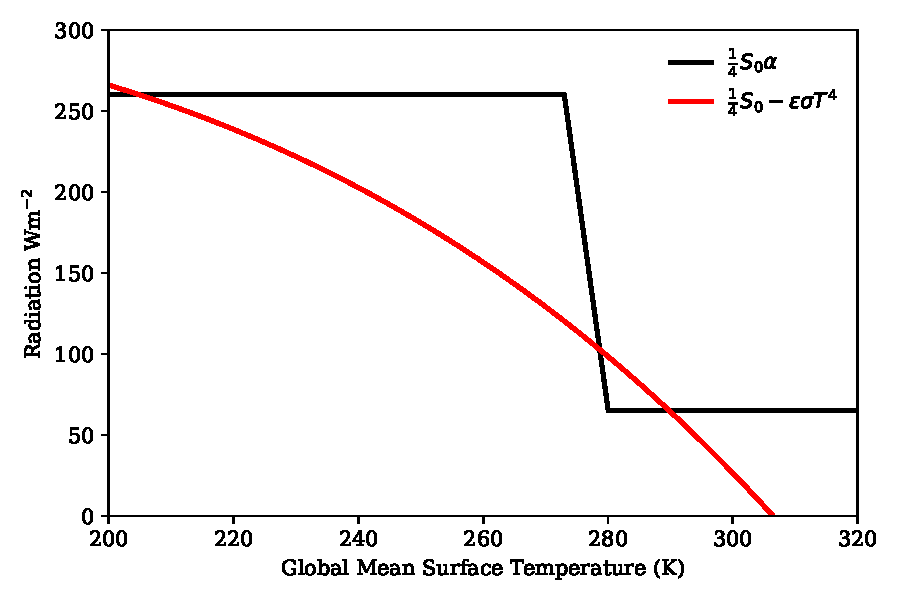
\includegraphics[width=\textwidth,keepaspectratio]{snowball}
  \caption{The solutions to \cref{eq:energy_balance,eq:snowball_earth_albedo} are given by the intersections of these curves. The solution at $T\approx\SI{210}{\kelvin}$ is the snowball
    state and the solution at $T\approx \SI{290}{\kelvin}$ is the present day state. The intermediate state can be shown to be unstable and as such is not physically observable. The parameters were
    chosen somewhat arbitrarily,  but give a good approximation to the present day state. The parameters are $\alpha_+ = 0.8,\alpha_-=0.2,\epsilon=0.65,T_0 = \SI{280}{\kelvin},S_0 = \SI{1300}{\watt\per\meter\squared}$
    and $\sigma = \SI{5.67e-8}{\watt\per\meter\squared\per\kelvin\tothe{4}}$.}
  \label{fig:energy_balance_solution}
\end{figure}

This snowball state was predicted without empirical evidence, however decades after it was postulated evidence arose for its existence \parencite{Kirschvink1992,Hoffman2002}.
This state appears to have existed in the Neoproterozoic around \SI{650}{\mega\year\beforepresent}.
There is evidence for glaciers near the equator during this time. It is not clear
if the Earth was totally covered in ice, or if there was a think equatorial ocean, leading to a `slushball' Earth, rather than a `Hard Snowball' \parencite{Pierrehumbert2005,Pierrehumbert2011}.

\subsubsection{Dansgaard-Oeschger Events}
Less dramatic warm/cold transitions exist within the Earth system. During the Quaternary period, the Earth existed in interglacial and glacial states \parencite{Lisiecki2005}. Within the last glacial period,
around \SIrange{100}{10}{\kilo\year\beforepresent}, there were rapid transitions between cool stadial and warmer interstadial states \parencite{Oeschger1984,Dansgaard1993}. These transitions were discovered
in ice cores from Greenland, and represent rapid (on the timescale of 10 years) warming, some of which are up to \SI{16.5}{\kelvin} \parencite{Kindler2014}. However the relaxation period
back to the stadial state is longer, occurring on centennial timescales. A record of the Dansgaard-Oeschger events is plotted in \cref{fig:ngrip}. There is evidence that these Dansgaard-Oeschger events
had a global impact as ice core records show synchronous changes in Antarctica \parencite{Buizert2015}.

\begin{figure}
  \centering
  \includegraphics[width=\textwidth,keepaspectratio]{ngrip}
  \caption[NGRIP record of Dansgaard Oeschger events]{A record of $\delta \ce{^{18}O}$ from the NGRIP ice core from Greenland \parencite{NGRIP2004} over the last $100,000$ years.
    Higher values correspond to warmer temperatures. The clear spikes in this record are Dansgaard-Oeschger events. Note the rapid warming and slower cooling.}
  \label{fig:ngrip}
\end{figure}

There is no consensus on the mechanisms of the Dansgaard-Oeschger events, but they are generally believed to be caused by the subtle interplay of atmospheric, sea ice and AMOC dynamics
\parencite{Vettoretti2022,Boers2018,Riechers2023arxiv}. There is ongoing debate about the nature of the transition observed in Dansgaard Oeschger events, with different researchers arguing
that Dansgaard Oeschger events are driven stochastically \parencite{Ditlevsen2010,Ditlevsen1999} or deterministically \parencite{Boers2018a}.

\subsubsection{Green Sahara}
In the more recent past, a different sort of abrupt shift happened involving the biosphere. During the early part of the Holocene there was a northward expansion of shrub and savannah ecosystems
into what was the Sahara desert, as revealed in the pollen record \parencite{Hoelzmann1998,Hely2014}. This is therefore a `greening' of the Sahara. It was a time of enhanced rainfall \parencite{Tierney2017}
and is termed the African Humid Period.

The African Humid Period came to an end between \SIrange{6000}{4000}{\year\beforepresent}. Different reconstructions \parencite{Shanahan2015,Kropelin2008} disagree on how abrupt the transition
was, which may relate to the different regions involved in the reconstruction. An explanation for this 
involves a biogeophysical feedback proposed by Jule Charney \parencite{Charney1975,Charney1975a}. The mechanism is that vegetated ground has a lower
albedo than non-vegetated ground, so decreasing the vegetation increases the albedo, leading to decrease in net incoming radiation and a radiative cooling of the atmosphere, and so the air sinks by adiabatic compression
which inhibits convection and thus rainfall. This decrease in rainfall would then cause a further vegetation decrease.

Some climate models \parencite{Renssen2006} found that the transition was not abrupt. However, more recent work \parencite{Hopcroft2021} using a model that was tuned with mid-Holocene data was able to simulate an abrupt
transition.

\section{A Typology of Tipping Points}
\label{sec:tipping_typology}
Having demonstrated the relevance of tipping points to the past and future of the Earth system I will continue with a more theoretical look at tipping points. It is helpful
to classify tipping according to a typology developed by~\cite{Ashwin2012}. They identified three types of tipping:
\begin{description}
\item[B-tipping] which refers to a tipping caused by a bifurcation in the underlying attractor of the system due to a change in a parameter of the system.
\item[N-tipping] which refers to a tipping caused by noisy fluctuations driving the system  from one attractor to another.
\item[R-tipping] which  refers to a tipping caused the system failing to track its continuously changing attractor. The `R' is for `rate' because the attractor is changing too
  fast for the system to adapt to it.
\end{description}

Since then, other researchers have found it useful to consider additional types of tipping. For example,~\cite{Halekotte2020} introduced the concept of shock or S-tipping which is when a single large perturbation
can push the system into a new state. When the system's attractor is not a steady state but is instead a limit cycle, the tipping can depend on the phase of the cycle, a phenomenon which has
been dubbed P-tipping \parencite{Alkhayuon2021}. 

A more detailed examination of B,N,R and S tipping will now be given.

\subsection{B-Tipping}
\label{sec:btipping}
\subsubsection{Theory}
Consider a system with a state variable $\bm{x} \in \mathbb{R}^n$ described by the system of ordinary  differential equations
\begin{equation}
  \label{eq:generic_system}
  \dv{\bm{x}}{t} = \bm{f}(\bm{x}).
\end{equation}
Suppose the system has a fixed point at $\bm{x}^*$, such that $\bm{f}(\bm{x}^*)=0$ then the linear stability of the system \parencite{Strogatz2015} is characterised by
the behaviour of a small perturbation $\bm{y}$ about this fixed point, where $\bm{y} = \bm{x} - \bm{x}^*$. Then the dynamics of $\bm{y}$ are governed by
\begin{equation}
  \label{eq:linearised_equation}
  \dv{\bm{y}}{t} = J\bm{y} 
\end{equation}
where terms of order $\mathcal{O}\left(\left|\bm{y}\right|^2\right)$ or higher have been neglected and $J$ is a matrix called the Jacobian defined by
\begin{equation}
  \label{eq:jacobian}
  J_{ij} = \eval{\pdv{\bm{f}_i}{\bm{x}_j}}_{\bm{x}=\bm{x}^*}.
\end{equation}
The solution to \cref{eq:linearised_equation} is
\begin{equation}
  \label{eq:solution_to_linearised_equation}
  \bm{y} = e^{tJ}\bm{y}(0).
\end{equation}
Suppose $J$ has $n$ linearly independent eigenvectors (although similar conclusions will hold if it does not \parencite{guckenheimer2013}).
Let the eigenvectors be $\{\bm{v}_i\}$ and the eigenvalues $\{\lambda_i\}$ then \cref{eq:solution_to_linearised_equation} can be written as
\begin{equation}
  \label{eq:solution_to_linearised_equation_eigen}
  \bm{y} = \sum_i c_i e^{t\lambda_i}\bm{v}_i
\end{equation}
where $\{c_i\}$ are a set of constants chosen to match the initial condition. It can be seen then that the long-time behaviour of $\bm{y}$ is
$\bm{y} \sim c_k e^{t\lambda_k} \bm{v}_k$ where $\lambda_k$ is the eigenvalue with largest real part. If this is positive, then $\bm{y}$ will leave the vicinity of $\bm{x}^*$ whereas
if it is negative $\bm{y}$ will approach $\bm{x}^*$. Suppose $\bm{x}^*$ is a hyperbolic fixed point, which means that $J$ has no eigenvalues with zero real part. Then the Hartman-Grobman theorem
\parencite{Grobman1959,Hartman1960,Hartman1963} guarantees that the trajectories of $\bm{y}$ will be topologically conjugate --- that is to say qualitatively the same --- in some
neighbourhood of $\bm{x}^*$ to the trajectories of $\bm{x}$.  This means that $\bm{x}^*$ is linearly stable only when $J$ has eigenvalues with only negative real parts.
The directions $\bm{v}_k$ with $\Re \lambda_k < 0$ are known as stable directions (as the flow is attracted to the fixed point along these directions),
those with $\Re \lambda_k > 0$ are unstable directions \parencite{Strogatz2015}.

B- or Bifurcation-tipping refers to tipping which is driven by changes to the stability, or the loss altogether, of these fixed points.
A bifurcation is a concept from the mathematical theory of dynamical systems, introduced by~\cite{Poincare1885}.
It is used to describe a situation where the fixed points of a system qualitatively change as a control parameter is varied.

Consider a modification to \cref{eq:generic_system} where a control parameter $\mu \in \mathbb{R}$, which could for example be atmospheric $\ce{CO2}$, has been introduced
\begin{equation}
  \label{eq:generic_system_control_parameter}
  \dv{\bm{x}}{t} = \bm{f}_{\mu}(\bm{x}).
\end{equation}
The fixed points are described by $\bm{f}_{\mu}(\bm{x}^*) = 0$. By the Implicit Function Theorem \parencite{Spivak1965}, $\bm{x}^*$ is a smooth
function of $\mu$ except at points where $J$ has a zero eigenvalue, these points in $(\bm{x},\mu)$ space are known as bifurcation points.
Other bifurcation points can occur when a stable fixed point becomes unstable (or vice versa). In both cases an eigenvalue of $J$ must cross the imaginary
axis, i.e.\ have zero real part \parencite{guckenheimer2013}. As a result of this, the Hartman-Grobman theorem is not applicable and so a non-linear analysis must be undertaken.

Fortunately, there are techniques to deal with this, using the Center Manifold Theorem \parencite{Morris1977}, which can be stated loosely as
\begin{theorem}[Center Manifold Theorem]
  \label{thm:center_manifold_theorem}
  Let the eigenvalues, $\{\lambda_i\}$, of $J$ be divided into three sets such that $\spec J = \sigma_s \cup \sigma_u \cup \sigma_c$, where $\sigma_s = \{\lambda_i : \Re \lambda_i < 0\}$,
  $\sigma_u = \{\lambda_i : \Re \lambda > 0\}$ and $\sigma_c = \{\lambda : \Re \lambda = 0\}$.
  Let their respective eigenspaces be $E_s$, $E_u$ and $E_c$. Then there are stable and unstable invariant manifolds $W_s$  and $W_u$ tangent to $E_s$ and  $E_u$ at $\bm{x}^{*}$,
  and a center manifold $W_c$ tangent to $E_c$ at $\bm{x}^*$.
\end{theorem}
The upshot of this theorem is that the dynamics are now controlled by the center manifold. Suppose that the unstable manifold is empty (the most relevant case for tipping point research)
then \cref{thm:center_manifold_theorem} implies that the dynamics are topologically conjugate to
\begin{subequations}
  \label{eq:center_manifold_topological_equivalence}
  \begin{align}
  \dv{\bm{u}}{t} &= g(\bm{u}) \\
  \dv{\bm{v}}{t} &= -\bm{v}
  \end{align}
\end{subequations}
with $(\bm{u},\bm{v}) \in W_c \times W_s$. At long times $\bm{v} \rightarrow \bm{0}$ so at long times the dynamics are given by $\bm{u}$ on the center manifold
\parencite{guckenheimer2013}. In order to calculate $g$, suppose that
$\bm{x} = (\bm{w},\bm{z}) \in \mathbb{R}^n$ so that
\begin{subequations}
  \label{eq:block_diagonal}
  \begin{align}
    \dv{\bm{w}}{t} &= A\bm{w} + p(\bm{w},\bm{z}) \\
    \dv{\bm{z}}{t} &= B\bm{z} + q(\bm{w},\bm{z})
  \end{align}
\end{subequations}
where $A,B$ have eigenvalues with zero and negative real parts respectively and $p,q$ are at least quadratic. Then the center manifold can be written as a graph $W_c = (\bm{w},h(\bm{w}))$
with $\bm{z} = h(\bm{w})$, so that on the center manifold
\begin{equation}
  \label{eq:dynamics_on_the_center_manifold}
  \dv{\bm{w}}{t} = A\bm{w} + p\left(\bm{w},h\left(\bm{w}\right)\right).
\end{equation}
The next step is to make \cref{eq:dynamics_on_the_center_manifold} as simple as possible. By the Hartman-Grobman theorem, \cref{eq:dynamics_on_the_center_manifold}
cannot be linearised. However the `next best' thing are normal forms, which describe the different sorts of possible bifurcations \parencite{Dijkstra2011}.

Consider again \cref{eq:generic_system_control_parameter}, but now enlarge the state space to $\mathbb{R}^{n+1}$ by viewing $\mu$ as a dynamic variable with $\dot{\mu} = 0$. Suppose
further, without loss of generality, that there is a bifurcation point at $(\bm{x},\mu)  = (\bm{0},0)$ where $J$ has a simple zero eigenvalue.
Then using \cref{thm:center_manifold_theorem} a center manifold passing through
$(\bm{0},0)$ can be found. If the trajectories are restricted to the center manifold and certain transversality conditions are met ($\partial_{\mu}f \neq 0,\partial_{xx} f\neq 0$ at the
bifurcation point) the the trajectories will be topologically equivalent \parencite{guckenheimer2013} to
\begin{equation}
  \label{eq:saddle_node}
  \dv{x}{t}  = \mu + x^2.
\end{equation}
This type of bifurcation is known as a saddle-node or a fold bifurcation.
This remarkable fact has simplified a high dimensional dynamical system to a generic one-dimensional one near the bifurcation point \parencite{Glendinning1994}.

The saddle-node bifurcation is very important as other bifurcation problems can be perturbed into a saddle-node bifurcation problem (as it is unusual for the transversality conditions
not to be met). In this sense, saddle-nodes are the type of bifurcations to be expected in nature. However if the transversality conditions are not met other sorts of bifurcations can arise.

If $\partial_{\mu}f=0$, then the bifurcation is equivalent to
\begin{equation}
  \label{eq:transcritical}
  \dv{x}{t} = \mu x - x^2,
\end{equation}
which is a transcritical bifurcation. If $\partial_{\mu}f = 0$ and $\partial_{xx}f=0$ with $\partial_{xxx}f \neq 0$ the bifurcation is known as a pitchfork bifurcation with normal form
\begin{equation}
  \label{eq:pitchfork}
  \dv{x}{t} = \mu x - x^3.
\end{equation}

Another important sort of bifurcation is a Hopf bifurcation \parencite{Hopf1942}. In this bifurcation a complex conjugate eigenvalue pair become purely imaginary, $\lambda = \pm i\omega$.
As there are no zero eigenvalues the Implicit Function Theorem implies no new equilibria will be created. However it will lead to a change in the dimensions of the
stable and unstable manifolds, leading to a qualitative change in the behaviour of the system. It can be shown that there is a center manifold on which a limit cycle can exist
\parencite{guckenheimer2013}. In other words, these bifurcations lead to the creation of periodic oscillatory behaviour. These bifurcations
can occur only in systems of dimension two or higher. The normal form of this bifurcation \parencite{Kuznetsov2004} can be expressed as a differential equation involving the complex variable $z = x + iy$
\begin{equation}
  \label{eq:hopf}
  \dv{z}{t} = (\mu + i) z - z|z|^2.
\end{equation}

\subsubsection{Example}
As an example of B-tipping, consider Stommel's AMOC model \parencite{STOMMEL1961}, which after a rescaling \parencite{Dijkstra2011} can be written as:
\begin{subequations}
  \label{eq:stommel_amoc}
  \begin{align}
    \dv{T}{t} &= \eta_1 - T\left(1 - \left|\Psi\right|\right) \\
    \dv{S}{t} &= \eta_2 - S\left(\eta_3 + \left|\Psi\right|\right) \\
    \Psi      &= T - S
  \end{align}
\end{subequations}
where $T$ and $S$ are (dimensionless) equator to pole temperature and salinity differences respectively.
The flux $\Psi = T - S$ is the strength of the AMOC. The parameters $\eta_1,\eta_2,\eta_3$ represent
thermal forcing, freshwater forcing and the ratio of their timescales respectively.

As $\eta_2$ is increased the strength of the AMOC decreases until it reaches a saddle-node bifurcation point
at $\eta_2^*  \approx 1.2$ where the AMOC abruptly transitions to a weaker state with flow in the opposite direction,
this is shown in \cref{fig:stommel_amoc}. Near the bifurcation point, the flux behaves like $\Psi \sim \sqrt{\eta_2^*-\eta_2}$,
which reflects the normal form \cref{eq:saddle_node}. If $\eta_2$ were to be decreased with the AMOC in the other state, $\eta_2$ would have to be decreased below
$\eta_2^*$ to the lower value $0.9$ to transition back into its original state.


\begin{figure}
  \centering
  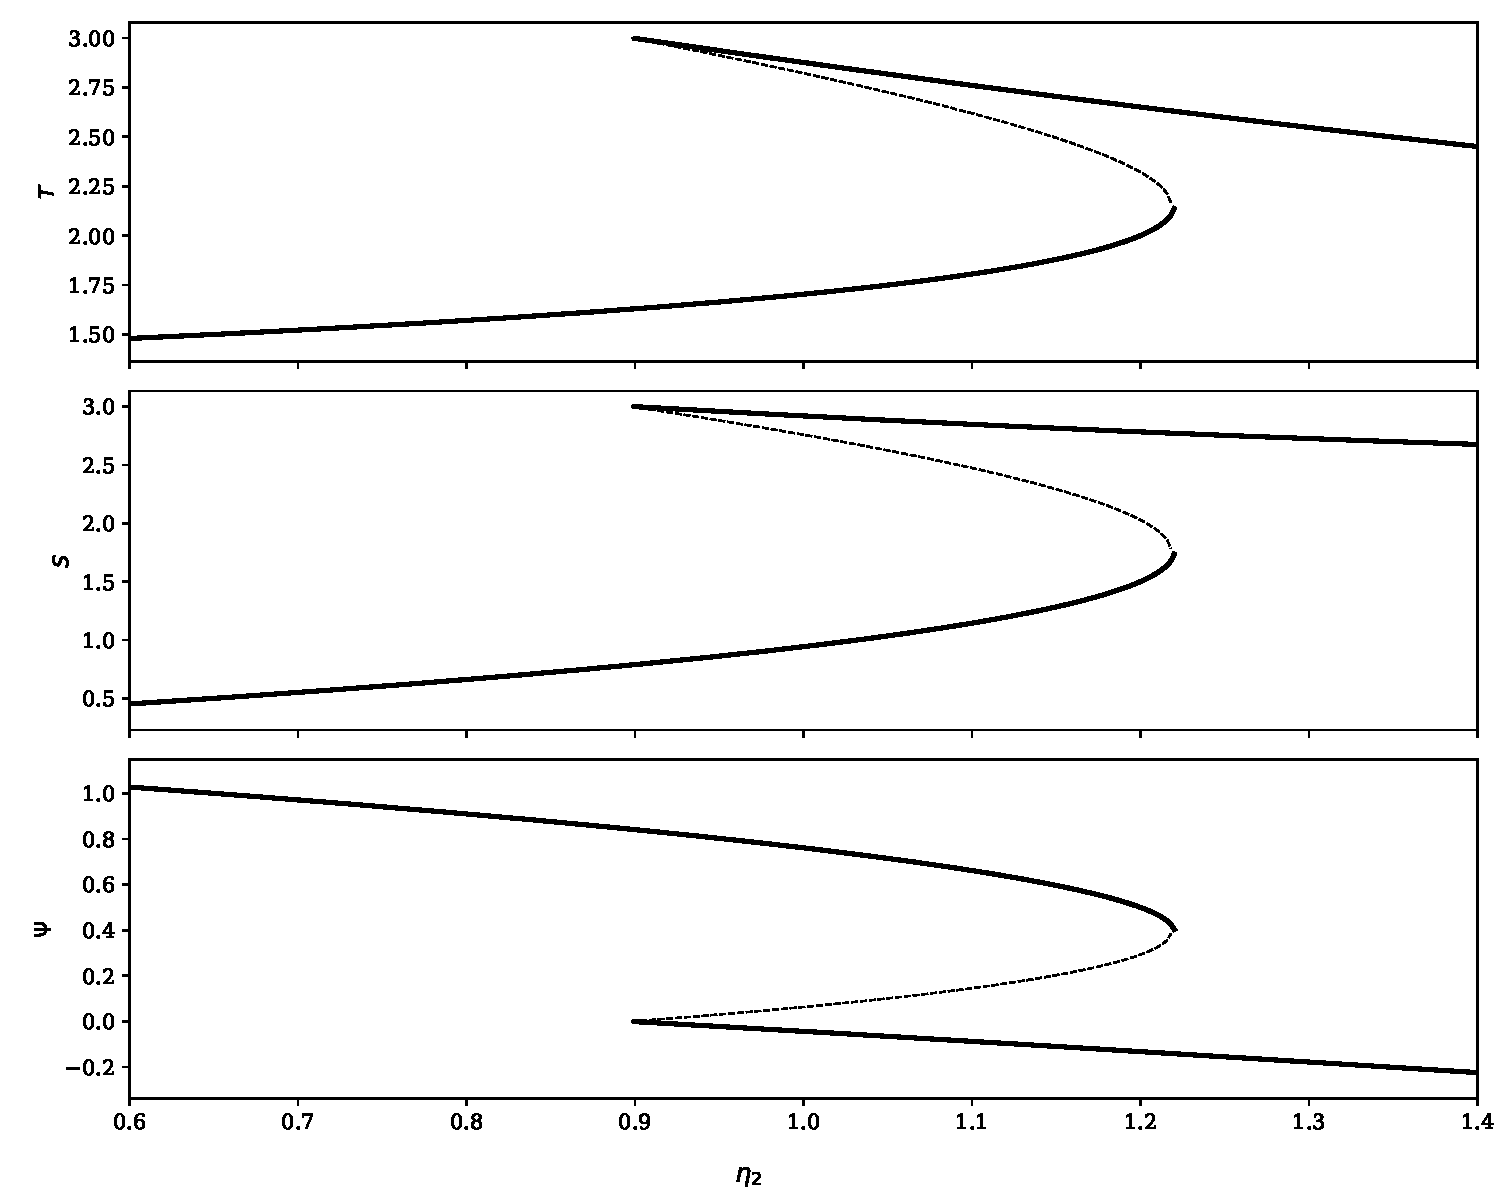
\includegraphics[width=\textwidth,keepaspectratio]{stommel}
  \caption[The Stommel Model of the AMOC]{The equilibrium states of the Stommel model, \cref{eq:stommel_amoc}, as a function of $\eta_2$. The stable states are given in solid lines,
    the unstable are given as a dashed line. As $\eta_2$ is increased, the AMOC transitions from a strong poleward flow to a weaker equatorward state. Note that near the
    bifurcation point around $\eta_2 \approx 1.2$ the stable states seem to behave like the square root of the control parameter. This reflects the normal form of
    the bifurcation. The parameters were set to $\eta_1 = 3,\eta_3=0.3$.}
  \label{fig:stommel_amoc}
\end{figure}
\subsection{N-tipping}
If a system with multiple stable states is subject to stochastic forcing, then it will perform transitions between these states if observed for long enough. This
phenomenon is called N- or noise-tipping. This has an important difference to B-tipping. In B-tipping an external driver changes a control parameter, causing a system to tip
but in N-tipping the natural variability of the system causes it to tip.

The role of noise in the climate system was identified by~\cite{Hasselmann1976}. He viewed the `slow' components of the earth system (the ocean, the vegetation and the ice sheets) as being
deterministic and the `fast' components (the atmosphere) as being essentially stochastic. This stochasticity may be viewed as an effective model for chaotic systems \parencite{Lorenz1963}
or resulting from unresolved processes \parencite{Palmer2009}. Certain paleoclimate abrupt shifts, such as the Dansgaard-Oeschger events, have been viewed a N-tipping \parencite{Ditlevsen1999}.

Stochastic differential equations can be written \parencite{Jacobs2010} as
\begin{equation}
  \label{eq:general_sde}
  \dv{\bm{x}}{t} = \bm{F}(\bm{x}) + G(\bm{x})\bm{\eta}(t),
\end{equation}
where a physicist's notation has been used. The vector function $\bm{F}$ represents the deterministic evolution and the matrix function $G$ represents the stochastic evolution. The function
$\bm{\eta}(t)$ is the source of the stochasticity. It has mean zero and is `delta correlated' in time, by which is meant
\begin{equation}
  \label{eq:eta_correlation}
  \E\left(\bm{\eta}_i(t)\bm{\eta}_j(t')\right) = \delta_{ij}\delta(t-t')
\end{equation}
where $\delta_{ij}$ is the Kronecker delta and $\delta(t-t')$ is the Dirac delta function.

Viewing individual solutions of \cref{eq:general_sde}, or sample paths, is one approach  to analysing stochastic systems. Another useful approach is to calculate the probability density function
(pdf), $p(\bm{x},t)$ of $\bm{x}$ and how it evolves in time. The tool to do this is the Fokker-Planck equation \parencite{Fokker1914,Planck1917}, given by
\begin{equation}
  \label{eq:fokker_planck}
  \pdv{p}{t} = - \sum_i \partial_i \bm{F}_i p + \sum_i\sum_j \partial_i\partial_j D_{ij} p
\end{equation}
where $D = GG^T/2$.

\subsection{Kramer's Escape Rate}
Often a very simple one-dimensional model is used in studies of N-tipping
\begin{equation}
  \label{eq:simple_sde}
  \dv{x}{t} = -\dv{U}{x} + \sigma \eta(t).
\end{equation}
This is an example of a potential system because it gives the deterministic dynamics as the gradient of a potential, $U(x)$. This can be done for any one dimensional system but is not
always the case for a higher dimensional system. Furthermore, the noise is assumed to be `white', with constant variance $\sigma^2$. It is known as white noise because in the frequency domain, all
frequencies are excited with equal amplitude. This is a questionable assumption for the Earth System, where the spectrum is not white \parencite{Mitchell1976,VonderHeydt2021} and may
change due to climate change \parencite{Huntingford2013}.

\Cref{eq:simple_sde} has an associated Fokker-Planck equation
\begin{equation}
  \label{eq:fokker_planck_one_d}
  \pdv{p}{t} = \pdv{x} \dv{U}{x}p + \frac{1}{2}\sigma^2 \pdv[2]{p}{x},
\end{equation}
which can also be written in the form of a continuity equation
\begin{equation}
  \label{eq:fokker_planck_continuity}
  \pdv{p}{t} + \pdv{J}{x} = 0
\end{equation}
where $J$ is the probability current given by
\begin{equation}
  \label{eq:probability_current}
  J(x) = -\dv{U}{x}p - \frac{1}{2}\sigma^2 \pdv{p}{x}.
\end{equation}

If \cref{eq:simple_sde} has multiple stable states, then and estimate of the transition rate between these states can be made. This estimate known
as the Kramers Rate \parencite{Kramers1940}. This derivation follows~\cite{Risken1984}.

\begin{figure}
  \centering
  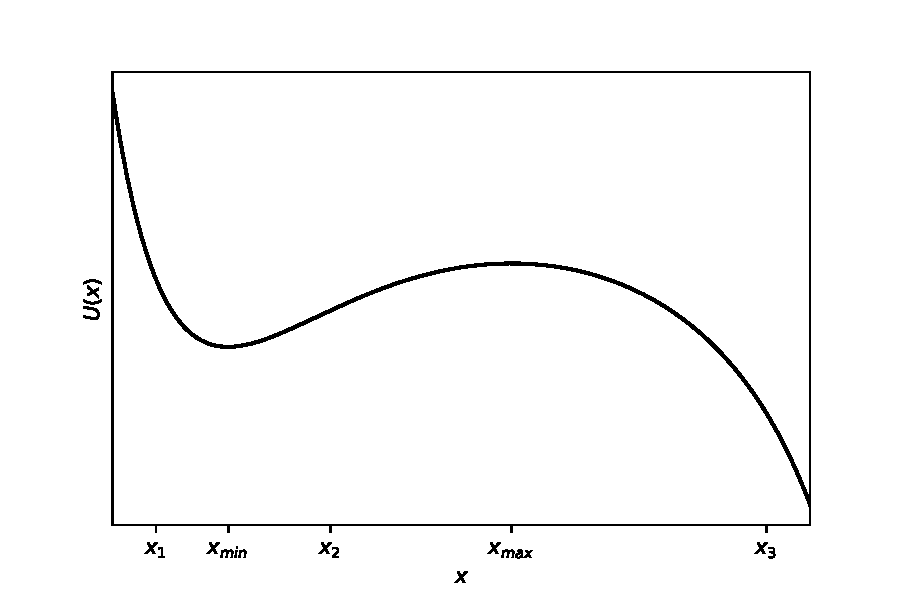
\includegraphics[width=\textwidth,keepaspectratio]{potential_to_escape}
  \caption{An example of a potential with a stable state at $x_{min}$ from which a system can escape over the potential barrier at $x_{max}$ to a new state near $x_3$.
  The precise locations of $x_1,x_2,x_3$ do not matter at the level of approximation Kramer's escape rate formula works at.}
  \label{fig:potential_to_escape}
\end{figure}

Suppose that $U$ has the form given by \cref{fig:potential_to_escape}, which has a stable state at $x_{min}$, an unstable state at $x_{max}$ and the rate at which the system
transitions from near $x_{min}$ in the region between $x_1$ and $x_2$ to near $x_3$ is to be determined. Assuming the system is in a near steady state, \cref{eq:fokker_planck_continuity}
implies that $J$ is approximately constant. Noting that $J$ can be put into the form
\begin{equation}
  \label{eq:probability_current_other_form}
  J = -\frac{1}{2}\sigma^2 e^{-\frac{2U(x)}{\sigma^2}} \pdv{x} \left( p(x) e^{\frac{2U(x)}{\sigma^2}}\right),
\end{equation}
which can then be integrated from $x_{min}$ to $x_3$ give
\begin{equation}
  \label{eq:integrated_J}
  J = \frac{\sigma^2}{2} \left(p(x_{min})e^{\frac{2U(x_{min})}{\sigma^2}} - p(x_3)e^{\frac{2U(x_{3})}{\sigma^2}}\right)\left(\int_{x_{min}}^{x_{3}} e^{\frac{2U(x)}{\sigma^2}} \dd{x}\right)^{-1}.
\end{equation}
As it will be rare to find the system at $x_3$, $p(x_3)$ is negligible. To estimate $p(x_{min})$, assume this is given by the equilibrium distribution which can be found by setting $J$ to
a constant. This constant can be chosen to be the value of $J$ at $x_{min}$, giving the following expression for the equilibrium pdf, $p_{eq}$,
\begin{equation}
  \label{eq:equilibrium_pdf}
  p_{eq}(x) = p(x_{min})e^{\frac{2U(x_{min})}{\sigma^2}}e^{-\frac{2U(x)}{\sigma^2}}.
\end{equation}
The probability of finding the system near $x_{min}$ is therefore
\begin{equation}
  \label{eq:p_near_xmin}
  \mathbb{P} = \int_{x_1}^{x_2} p_{eq}(x) \dd{x} = p(x_{min})e^{\frac{2U(x_{min})}{\sigma^2}} \int_{x_1}^{x_2} e^{-\frac{2U(x)}{\sigma^2}} \dd{x}.
\end{equation}
The escape rate is $r = J/\mathbb{P}$ which becomes
\begin{equation}
  \label{eq:escape_rate_integrals}
  r^{-1} = \frac{2}{\sigma^2} \int_{x_1}^{x_2} e^{-\frac{2U(x)}{\sigma^2}} \dd{x} \int_{x_{min}}^{x_3} e^{-\frac{2U(x)}{\sigma^2}} \dd{x}.
\end{equation}
Each integral can be asymptotically evaluated using Laplace's Method \parencite{Bender1978} to give Kramers escape rate
\begin{equation}
  \label{eq:kramers}
  r^{-1} \sim \frac{2\pi}{\sqrt{U''(x_{min})|U''(x_{max})|}} e^{\frac{2}{\sigma^2}\left(U(x_{max})-U(x_{min})\right)},
\end{equation}
for $ \sigma \rightarrow 0$.

\subsubsection{Example}
As an example consider the potential
\begin{equation}
  \label{eq:example_potential}
  U(x) = -\frac{1}{2}x^2 + \frac{1}{12}x^4
\end{equation}
which has symmetric stable states at $x = \pm \sqrt{3}$. There is a potential barrier at $x = 0$. Assuming that $\sigma = 0.75$, Kramer's rate predicts a transition
timescale of $r^{-1} \approx 65$ time units. \Cref{fig:ntipping} shows transitions happening on this timescale.

\begin{figure}
  \centering
  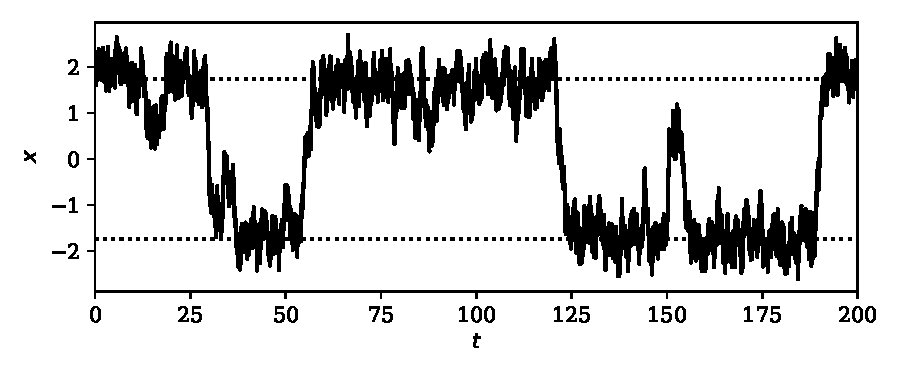
\includegraphics[width=\textwidth,keepaspectratio]{noise_trans}
  \caption[An example of N-tipping]{A time series showing transitions between two stable states (indicated by a dotted line). Kramers formula, \cref{eq:kramers} predicts a
    transition timescale of about $65$ time units. The time series shows transitions happening on this timescale.}
  \label{fig:ntipping}
\end{figure}


\subsection{R-tipping}
A relatively recently discovered type of tipping is R-tipping. First discovered by~\cite{Luke2011} in a simple model of soil temperatures, R-tipping or rate-tipping refers to
a situation where the rate of change of a control parameter, rather than the magnitude of the parameter itself  controls whether a system tips or not \parencite{Perryman2014a}.
This type of tipping occurs in nonautonomous dynamical systems, which is a system with explicit time dependence \parencite{Ashwin2017a}.

This sort of tipping is best explained through an example, taken from~\cite{Ashwin2012}. The system is
\begin{subequations}
  \label{eq:rtipping_example}
  \begin{align}
    \dv{x}{t}   &= \left(x + \mu\right)^2 - 4 \label{eq:rtipping_example_x} \\
    \dv{\mu}{t} &= r.                          \label{eq:rtipping_example_r} 
  \end{align}
\end{subequations}
These equations can be interpreted as a system with state $x$ in a changing environment represented by parameter $\mu$ that changes at some finite rate, $r$.

\begin{figure}
  \centering
  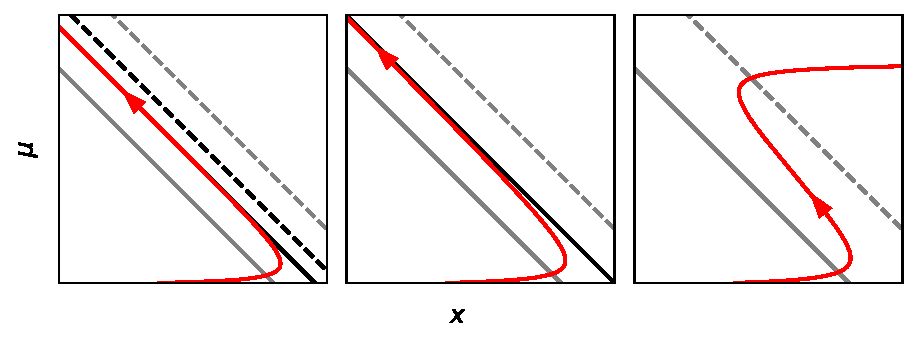
\includegraphics[width=\textwidth,keepaspectratio]{rate}
  \caption[R-tipping mechanism]{Panels showing the state space of a system, \cref{eq:rtipping_example}, undergoing R-tipping.
    From left to right, the figures show the system below the critical rate, at the critical rate and above the critical rate. In the left panel, with $r=3.2$ the lines
    $x^{\mathrm{PB}}_{\pm}$ exist and are separated. In the center panel with $r = r_c = 4$, $x^{\mathrm{PB}}_{\pm}$ exist and have collided into one line. In the right panel,
    $r = 4.8$ and therefore $x^{\mathrm{PB}}_{\pm}$ do not exist. As a result trajectories diverge as the system has undergone R-tipping. Note that for all values of $r$, the
    quasi-static equilibria exist.}
  \label{fig:rate_tipping}
\end{figure}

Consider the `frozen system' \parencite{Wieczorek2021}, which is \cref{eq:rtipping_example_x} with $\mu$ constant --- this describes the dynamics
in the case where the environment is unchanging. It has equilibria at
$x^*_{\pm} = \pm 2 - \mu$. The stability of these equilibria can be found in the manner described in \cref{sec:btipping}, which in this case amounts to evaluating
the derivative of \cref{eq:rtipping_example_x} with respect to $x$ at $x^*_{\pm}$. These quasi-static equilibria are shown as grey lines in \cref{fig:rate_tipping}, where
the stable quasi-static equilibria are shown in solid grey and the unstable quasi-static equilibria are shown as a dashed line.
It can be shown that $x_-$ is stable for all $\mu$ values, and $x_+$ is unstable for all $\mu$ values. As a result a na{\"i}ve B-tipping analysis
would suggest this system cannot tip. However, as will be shown, this system can undergo R-tipping.

To see this, make a change of coordinates into a co-moving frame by setting $y = x + \mu$. Then the system becomes
\begin{equation}
  \label{eq:rtipping_co_moving}
  \dv{y}{t} = y^2 + r - 4.
\end{equation}
This equation has a stable fixed point at $-\sqrt{4-r}$ and an unstable fixed point at $\sqrt{4-r}$. Returning to the $x$ coordinates these solutions correspond to the
pullback attractor and repeller of the system, $x^{\mathrm{PB}}_{\pm} = \pm \sqrt{4 - r} - \mu$. These pullback objects are the appropriate generalisation of attractors and repellers to the
nonautonomous case \parencite{Ghil2020a}. They are plotted in black in \cref{fig:rate_tipping} where the solid line
is the stable state and the dashed line is unstable. It is to $x_-^{\mathrm{PB}}$ rather than $x_-$ that the solutions of \cref{eq:rtipping_example} are attracted to, plotted in red
in \cref{fig:rate_tipping}.

If $r < 4$, then $x_-^{\mathrm{PB}}$ exists and so solutions evolve towards it. However if $r > 4$ then $x_-^{\mathrm{PB}}$ does not exist and so solutions diverge to infinity. As a result there
is a critical rate, $r_c = 4$, above which R-tipping occurs.

\subsubsection{Example}
The paradigmatic example of R-tipping is the Compost Bomb instability \parencite{Luke2011,Wieczorek2011,Clarke2021,OSullivan2022arxiv}, which is a thermal
instability in the soil. This phenomenon is caused by microbial respiration warming the soil, which in turn increases the soil temperature. However, this respiration decreases the supply
of soil carbon and thus decreases the amount of respiration and thus heating in the soil. Due to the differences between the (rapid) timescale of heating and the (slow) timescale of soil
carbon decrease there is the possibility for a dramatic increase in soil temperature.~\cite{Luke2011} found that if the air temperature raised faster than a critical rate then the
compost bomb instability would be caused. Their model was 
\begin{subequations}
  \label{eq:compost_bomb}
  \begin{align}
    \mu\dv{T_s}{t} &= -\lambda \left(T_s - T_a\right) + Ar_0 C_s e^{\alpha T_s} \\
    \dv{C_s}{t}    &= \Pi - r_0 C_s e^{\alpha T_s} \\
    \dv{T_a}{t}    &= \dot{T}_a
  \end{align}
\end{subequations}
where $T_s$ is the soil temperature, $T_a$ is the air temperature and $C_s$ is the soil carbon. The parameters, taken from~\cite{Wieczorek2011}, are a heat capacity
$\mu = \SI{2.5E6}{\joule\per\meter\squared\per\kelvin}$, a thermal coupling $\lambda = \SI{5.049E6}{\joule\per\year\per\meter\squared\per\kelvin}$, a heat of
respiration $A = \SI{3.9E7}{\joule\per\kilo\gram\carbon}$, a specific respiration $r_0 = \SI{0.01}{\per\year}$, a temperature dependence of respiration $\alpha = \SI{0.09}{\per\kelvin}$
and a net primary productivity $\Pi = \SI{1.055}{\kilo\gram\carbon\per\meter\squared\per\year}$. When the rate of increase in temperature was increased above a critical rate,
$\dot{T}_a \approx \SI{0.08}{\kelvin\per\year}$ the instability is triggered.

\begin{figure}
  \centering
  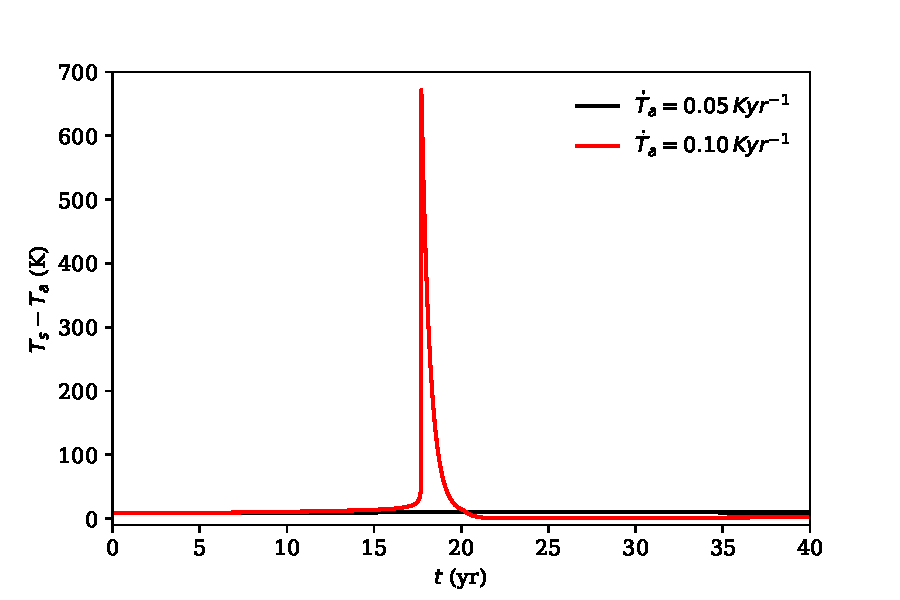
\includegraphics[width=\textwidth,keepaspectratio]{cbomb}
  \caption[Compost Bomb]{A plot of soil temperature relative to air temperature with two different rates of warming, calculated from \cref{eq:compost_bomb}. Note the spike in temperatures
  for high enough rates of warming---an example of R-tipping.}
  \label{fig:compost_bomb_example}
\end{figure}

\Cref{fig:compost_bomb_example} shows two time series of \cref{eq:compost_bomb} with $\dot{T}_a = \SI{0.05}{\kelvin\per\year}$ and $\dot{T}_a = \SI{0.1}{\kelvin\per\year}$. For the larger
rate of warming there is a clear spike in the soil temperatures.

\subsection{S-tipping}
A more recent addition to the tipping points typology is that of S- or shock-tipping. This refers to a situation where a single large perturbation
can push a system from one state to another \parencite{Halekotte2020,Feudel2023}, such as an extreme weather event on an ecosystem.
In this sense it is closely related to ideas of resilience introduced by~\cite{Holling1973}.

It is related to N-tipping but should be differentiated from it in the following sense. If $\bm{x}^*$ is a fixed point, with a basin of attraction $\mathcal{B}$ then the
smallest perturbation required to push the system into a new state is given by
\begin{equation}
  \label{eq:smallest_perturbation}
  \bm{\Delta} = \argmin \{ |\bm{x}'|^2 : \bm{x}^* + \bm{x}' \notin \mathcal{B}\}.
\end{equation}
If the system is the potential system \cref{eq:simple_sde}, then this is equal in magnitude to the distance to the nearest maximum, $|x_{max} - x_{min}|$. This should be compared to Kramer's formula,
\cref{eq:kramers}, which is a function of the difference in potential $U(x_{max}) - U(x_{min})$. In other words, S-tipping depends on the distance to the potential barrier, but N-tipping depends on
the height of that barrier.

\subsubsection{Example}
Consider a population growing via logistic growth with carrying capacity $k$ that is subject to the Allee Effect \parencite{Allee1932,Stephens1999}, which is an effect that reduces
growth rates at low population densities. A simple model of this is
\begin{equation}
  \label{eq:allee_effect}
  \dv{x}{t} = x\left(x-1\right)\left(1-\frac{x}{k}\right),
\end{equation}
where $k > 1$ and $x$ is a population density. This has equilibria at $x_1 = 0$, $x_2 = 1$ and $x_3 = k$. The equilibria $x_1,x_3$ are stable. $x_1$ corresponds to an extinct
state and $x_3$ to a populated state.

If the system is initially in equilibrium at $x_3$, the distance to the basin boundary is $\Delta = |x_3 - x_2| = k - 1$. Hence if the system receives a kick of
this magnitude or greater then the system will transition to the extinction state. In \cref{fig:shock_tipping}, \cref{eq:allee_effect} is integrated with $k = 2.0$ and given perturbations of
magnitude $0.99$ and $1.01$ at times $25.0$ and $50.0$. The first perturbation is not large enough to push the system across the boundary of the basin of attraction, yet the second one is
which is why the population undergoes S-tipping after the second perturbation.

\begin{figure}
  \centering
  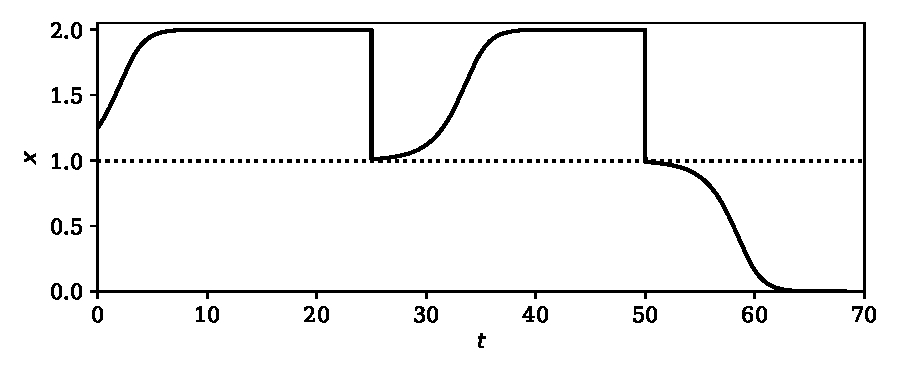
\includegraphics[width=\textwidth,keepaspectratio]{shock}
  \caption{An example of shock-tipping. The system given by \cref{eq:allee_effect} receives a perturbation of $0.99$ at time $25.0$. This is not large enough to make it cross the basin boundary
    (given by the dotted line) and so the system recovers. However at time $50.0$ a perturbation of $1.01$ is given which is enough to make it cross the basin boundary and thus to make the
  population go extinct.}
  \label{fig:shock_tipping}
\end{figure}

\subsection{Tipping in Reality}
This typology has given the impression that individual tipping phenomena can be easily assigned to the categories of B,N,R or S-tipping. However this is not the case as any
real tipping point will have aspects of many of the different tipping types. For example, If a control parameter is changing such that the system is approaching a B-tipping point,
then Kramer's formula \cref{eq:kramers} implies that the system is more likely to undergo N-tipping. Furthermore a system nearing a tipping point will be more likely to undergo S-tipping as
$\Delta$, defined by \cref{eq:smallest_perturbation}, is smaller as the basin of attraction shrinks. If a system is experiencing a shock, it is also likely that its parameters will
be changing quickly as well so this tipping will have an R-tipping character too.

Although real tipping points may have multiple characteristics it is still often possible and, more importantly, still useful to categorise the tipping into one of the above categories.


\section{Early Warning Signals}
Given the large impact a climate tipping point would have \parencite{Lenton2019a}, it would be useful to know at what level of climate forcing they would be triggered.
However models show little agreement about the level of forcing required to cause them \parencite{Drijfhout2015}. The processes of interest are by their nature
nonlinear and often involve interactions between the physical climate and the biosphere, where the `correct' equations are inherently uncertain. Furthermore,
some tipping behaviour may depend on subgrid scale processes, such as in the case of fire \parencite{Mangeon2016}. As a result a precise determination of the dangerous level of climate
forcing is challenging.

Instead, a theory of \emph{early warning signals} (EWS), sometimes known as  \emph{early warning indicators} (EWI), has emerged \parencite{Dakos2008,Scheffer2009,Lenton2011,Williamson2015}.
These techniques attempt to use certain generic statistical features of tipping points to provide an indication as to whether a system is
moving towards a tipping point. This is closely related to ideas about normal forms developed in \cref{sec:btipping}.

However not all types of tipping will give good early warning signals. Noise and shock tipping are not driven by a continuously changing external factor and
so early warning signals (in the conventional sense) will not be useful in these cases. For the case of rate tipping, there has been some work on
early warning signals \parencite{Ritchie2016}. However most of the work has been done
for bifurcation tipping where statistics can be calculated as a function of a slowly evolving parameter.

\subsection{Critical Slowing Down}
The basic idea of early warning signals is that of \emph{critical slowing down} \parencite{Dakos2008}. Suppose there is a system
\begin{equation}
  \label{eq:system}
  \dv{x}{t} = f(x,\mu)
\end{equation}
which has a stable state for $\mu < \mu_c$ at $x^*$ and undergoes a bifurcation when $\mu=\mu_c$. Then before the bifurcation, the system can be linearised about this steady state
to give
\begin{equation}
  \label{eq:linearised_about_steady_state}
  \dv{y}{t} = -\lambda y
\end{equation}
where $y = x -x^*$ and $\lambda = -f'(x^*,\mu)$. As the bifurcation is approached, $\lambda \rightarrow 0$ so any method that detects changes in $\lambda$ can act as an early warning
signal, in a quite generic way, for B-tipping.

Solving \cref{eq:linearised_about_steady_state} gives
\begin{equation}
  \label{eq:solved_linaer}
  y = e^{\lambda t} y(0)
\end{equation}
and so $\lambda^{-1}$ gives the timescale for perturbations to relax to equilibrium. This means that as $\lambda \rightarrow 0$,
this timescale approaches infinity, hence the name critical slowing down.


\subsection{Variance and Autocorrelation}
A very common way to approach early warning signals is to assume that the system of interest can be modeled as a one dimensional system subject to additive gaussian white noise. The first
of these assumptions is defensible on the grounds that near a bifurcation point, generic systems behave qualitatively like \cref{eq:saddle_node}. The second assumption is more suspect
as systems are generally subject to time correlated noise, such as red noise. However in the case of red noise, as long as the dynamics are considered over long enough timescales, then the
noise can be approximated as white. This assumption amounts to analysing the Langevin equation \parencite{Langevin1908}
\begin{equation}
  \label{eq:stochastic_system}
  \dv{x}{t} = f(x) + \sigma \eta(t) 
\end{equation}
where $\eta$ is delta correlated noise and $\sigma^2$ is the variance of the noise. This system can then be linearised to give
\begin{equation}
  \label{eq:ou_process}
  \dv{y}{t} = -\lambda y + \sigma \eta(t)
\end{equation}
where $y$ and $\lambda$ are defined as in \cref{eq:linearised_about_steady_state}. This is the equation that defines an Ornstein-Uhlenbeck process \parencite{Uhlenbeck1930} and its statistical
properties are well known. The Fluctuation-Dissipation Theorem \parencite{Marconi2008,Kubo1966,Leith1975,Einstein1905}
provides a link between the variability of a system and its response to
forcing, i.e. $\lambda$.

In this case the important statistics are
\begin{align}
  \sigma^2_y &= \frac{\sigma^2}{2\lambda} \label{eq:y_var}\\
  \alpha_1   &= e^{-\lambda} \label{eq:y_ac}
\end{align}
where $\sigma^2_y$ is the variance of $y$ and $\alpha_1$ is the autocorrelation of $y$ at lag 1. As $\lambda \rightarrow 1$
\begin{align}
  \sigma_y^2 &\rightarrow \infty \\
  \alpha_1    &\rightarrow 1.
\end{align}
This means that as a system with state $x$ approaches a B-tipping point, then its fluctuations about equilibrium, given by $y$, should have their variance diverge and their autocorrelation
tend to unity.

The question remains how to extract $y$ from a time series of $x$. If $x^*$, the equilibrium, was known then this could be directly subtracted from $x$ to give $y$. However if the equlibrium was known
then there would be no need for early warning signals as the bifurcation point could be calculated explicitly. Instead it is usually assumed that by subtracting a (possibly nonlinear) trend
off of $x$ what remains will approximate $y$.

This leads to the following method to generate early warning signals from a time series:
\begin{enumerate}
\item Split the time series of $x$ into rolling windows of length $\tau_w$. Let $x_i$ refer to the $x$ values in window $i$.
\item Detrend the time series $x_i$ to get $y_i$.
\item Calculate the variance $\sigma^2_{y_i}$ and autocorrelation $\alpha_{1}$ of $y_i$.
\item Perform statistical tests to detect if $\sigma^2_{y_i}$ and  $\alpha_{1}$ are increasing. Statistical tests, such as the Mann-Kendall test \parencite{Wilks2019} or a phase
  surrogate approach \parencite{Boettner2022} are commonly used.
\item If they are increasing, then this can be taken as an early warning of an approaching B-tipping. 
\end{enumerate}

In order for this technique to work, a particular assumption about timescales must be satisfied \parencite{Thompson2011b}. This is that
\begin{equation}
  \label{eq:timescale_separation}
  \tau_{\mathrm{drift}} \gg \tau_{\mathrm{crit}} \gg \tau_{\mathrm{stab}},
\end{equation}
which are the timescales of the long term drift of the system, the timescale of the critical direction of the system (which is the one being destabalised) and the other timescales of the stable directions
respectively. The first inequality is needed so that $\mu$ can be assumed to be constant in each sliding window. The second is needed so that the timescale being detected is the timescale corresponding
to the critical direction. It should be noted that $\tau_{\mathrm{crit}} \rightarrow \infty$ as the bifurcation is approached and so inequality \ref{eq:timescale_separation}
will be violated eventually. Furthermore anthropogenic climate change is happening on fast
timescales so it may be the case that $\tau_{\mathrm{drift}} \approx \tau_{\mathrm{crit}}$ or even $\tau_{\mathrm{drift}} \ll \tau_{\mathrm{crit}}$.

\subsubsection{Example}
In \cref{fig:ews} early warning signals are calculated for the system
\begin{equation}
  \label{eq:ews_system}
  \dv{x}{t} = x - \frac{1}{3}x^3 - \mu + \sigma \eta(t)
\end{equation}
where $\mu = \epsilon t$, $\sigma = 0.025$ and $\epsilon = 1\times 10^{-4}$. The value of $\epsilon$ has been chosen to be small to enable an autonomous analysis. The system has a bifurcation when $\mu = 2/3$.
The value of $\lambda$ can be calulated by taking a derivative:
\begin{equation}
  \label{eq:ews_lambda}
  \lambda = \left(x^*\right)^2 - 1 
\end{equation}
where $x^*$ is the equilibrium. The variance and autocorrelation are calculated as is the variance and autocorrelation calculated through \cref{eq:y_var,eq:y_ac}. It can be seen there is a
good agreement and a clear early warning signal before the bifurcation.
\begin{figure}
  \centering
  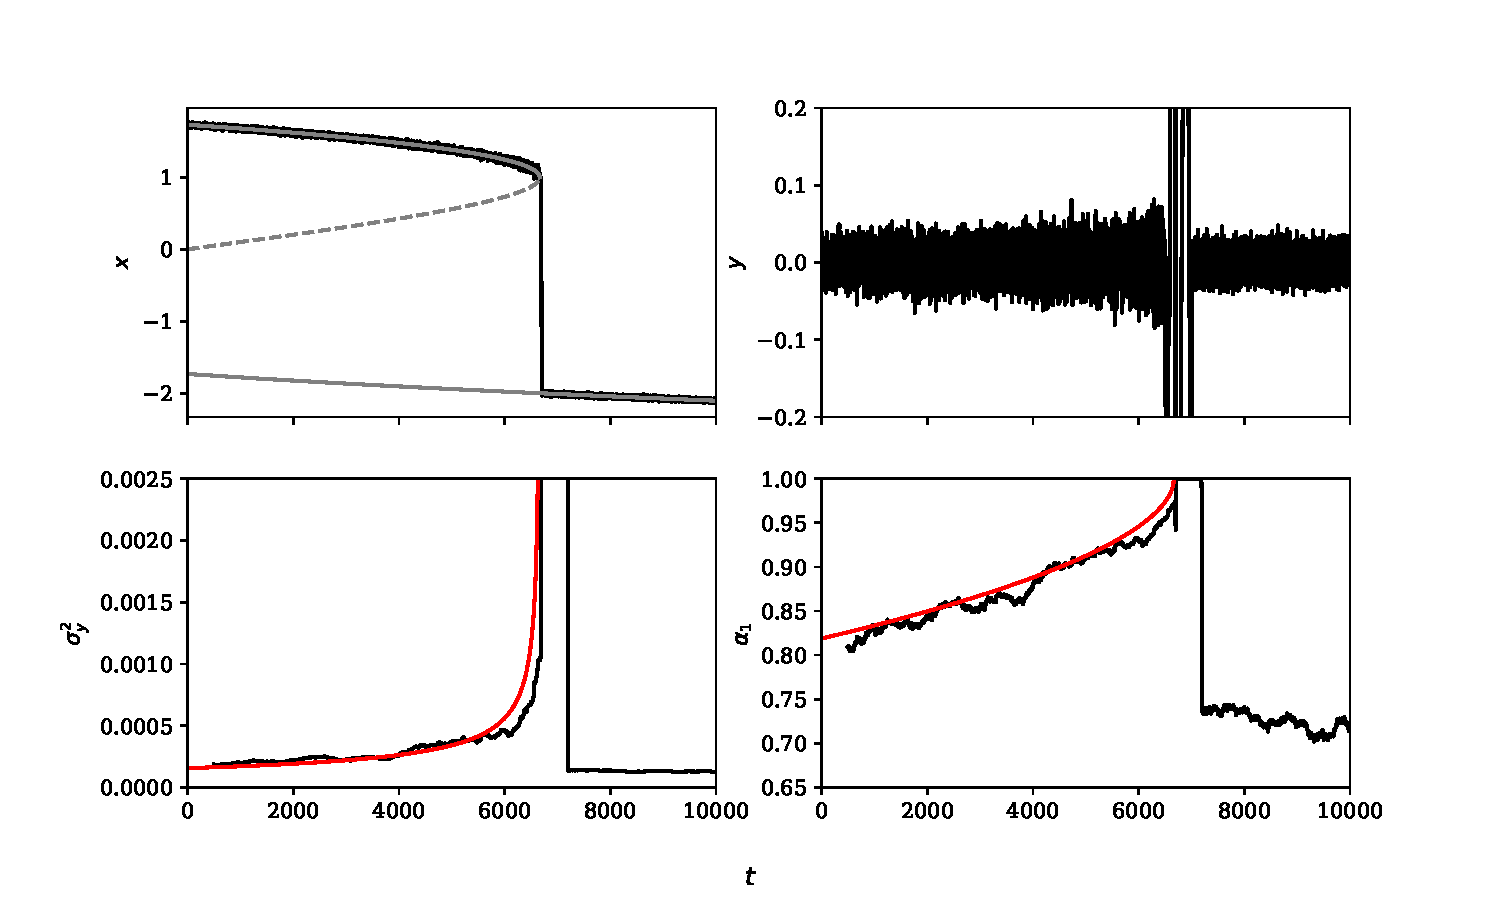
\includegraphics[width=\textwidth,keepaspectratio]{ews}
  \caption[An example of an early warning signal]{An example of using early warning signals to detect an approaching tipping point. In the top left is the original time series in black, obtained
    from integrating \cref{eq:ews_system} with a timestep of $0.1$. Also shown in grey are the quasi-static equilibria, where the unstable equilibria are shown with a dotted line.
    The top right shows the time series detrended using a cubic polynomial in windows of length 500 time units.
    The bottom left shows the variance of the detrened time series with the variance calculated through \cref{eq:y_var} in red. The bottom right shows the autocorrlation of the detrended time series
    with the autocorrelation calculated by \cref{eq:y_ac} shown in red. There is a clear early warning signal of rising variance and autocorrelation before the bifurcation.}
  \label{fig:ews}
\end{figure}

\subsection{Other Early Warning Signals}
These indicators have been generalised to higher dimensional and periodically forced systems \parencite{Williamson2015,Williamson2016}. Attempts have also been made to estimate
$\lambda$, the inverse timescale directly \parencite{Boettner2022,Boers2021a} The idea to look at
changes in timescale of fluctuations has been investigated using Detrended Fluctuation Analysis \parencite{Livina2007} where it was used to anticipate the warming at the
end of the Younger Dryas. Changes in these timscales can also lead to spectral reddening \parencite{Kleinen2003}. Higher order moments have prooved useful too, such as the
skewness \parencite{Guttal2008} and kurtosis \parencite{Xie2019}. The phenomenon of flickering \parencite{Wang2012}, in which systems `flicker' back and forth between alternative stable
states can also be used to detect upcoming transitions. More recently, machine learning techniques have had success in giving early warning for modelled transitions \parencite{Bury2021}.
Any measure of resilience of an ecosystem can function as an early warning indicator, see~\cite{Krakovska2023} for examples of ecological resilience.


Methods which calculate the early warning statistics over space rather than over time have also been used \parencite{Donangelo2010,Guttal2009}. Changes in spatial
patterns, for example of vegetation, have also been suggested as early warning indicators \parencite{Kefi2007,Kefi2014} although introducing spatial dynamics can complicate the analysis
of tipping points \parencite{Rietkerk2021}.

Whilst these indicators generally try to be generic --- in that they are applicable to many different systems --- there is no reason why early warning indicators cannot be designed for specific systems.
\cite{Parry2022} found that the seasonal cycle in temperature was a potential early warning system for Amazon dieback and~\cite{Boulton2013} found the sensitivity of net ecosystem productivity to temperature decreases
towards the tipping point.

\subsection{The Use of Early Warning Signals}
Early Warning Signals have been applied to the Earth system. For example~\cite{Dakos2008} applied them to a variety of abrupt shifts and found that they were preceded by rises in autocorrelation,
although some of these trends could have occured by chance. They have also been used to provide evidence for the subpolar gyre circulation detstabalising prior to the
Little Ice Age \parencite{Arellano-Nava2022}. Furthermore their presence has been
used to argue that Dansgaard-Oeschger events are B-tipping \parencite{Boers2018a} and their absence has been used to argue that Dansgaard-Oeschger events are N-tipping \parencite{Ditlevsen2010}.
These contradictory findings
are related to differences in the way the ice core data is processed.

Early Warning Signals have been investigated for the Greenland ice sheet \parencite{Boers2021}. This study suggeted the ice sheet was close to a tipping point.
However given the slow response of the ice sheet and
the fast change of the climate, inequality~\ref{eq:timescale_separation} is likely to be violated with the timescale of the drift to be much faster than the timescale of the dynamics.
Further more the analysis is of melt rates
rather than a state variable which describes the ice sheet itself. However the researchers could relate the observed fluctuations to a physically motivated simple nonlinear model of the ice sheet,
which would suggest the ice sheet is approaching a tipping point.

Later that year, another paper~\cite{Boers2021a}, was published suggesting the AMOC was approaching a tipping point due to increases in autocorrelation and variance.
Other work \parencite{Ditlevsen2022arxiv} went as far
as to suggest that most likely year for the AMOC to tip is 2067. Although the dynamics of the AMOC are faster than that of the ice sheets \parencite{ArmstrongMcKay2022}, it is still not clear if
inequaltiy~\ref{eq:timescale_separation} is satisfied but early warning signals have been used in complex models to detect AMOC shutdown \parencite{Boulton2014}.
Furthermore, the analysis was not based on the AMOC strength directly but on `fingerprints' derived from sea surface temperature and salinity data.

Recent work \parencite{Boulton2022} found increases in the autocorrelation in  the Vegetation Optical Depth (a satellite measure of vegetation biomass) in the Amazon,
which is consistent with a loss of resiliance in that
ecosystem. The results for changes in variance were more equivocal. Whilst the Amazon is a relatively fast tipping point \parencite{Ritchie2021}, some complex models do not show
generic early warning signals before the
tipping point \parencite{Boulton2013}. Other work \parencite{Fernandez-Martinez2023}, which examined global datasets of net biome productivity, did not find increasing autocorrelation
over the Amazon. However net biosphere productivity is a flux, not a state variable.